%
% 2-geometrie.tex
%
% (c) 2025 Prof Dr Andreas Müller
%
\section{Geometrische Eigenschaften% holomorpher Funktionen
\label{buch:holomorph:section:geometrie}}
\kopfrechts{Geometrische Eigenschaften holomorpher Funktionen}
Eine holomorphe Funktion $f(z)$ kann auch als Abbildung einer
offenen Teilmenge der komplexen Ebene auf die komplexe Ebene
betrachtet werden.
Reell differenzierbare Abbildungen von offenen Teilmengen von
$\mathbb{R}^2$ auf $\mathbb{R}^2$ können sehr komplizierte
Geometrie haben.
Die Cauchy-Riemann-Differentialgleichungen
für die Ableitungen von Real- und Imaginärteil einer holomorphen Funktion
schränken auch die geometrischen Eigenschaften einer solchen
Abbildung ein.
In diesem Abschnitt soll gezeigt werden, dass solche Funktionen
immer konform sind.

%
% 21-konform.tex -- Konforme Abbildungen
%
% (c) 2026 Prof Dr Andreas Müller
%
\subsection{Konforme Abbildungen}
%
% fig-konform.tex
%
% (c) 2026 Prof Dr Andreas Müller
%
\begin{figure}
\centering
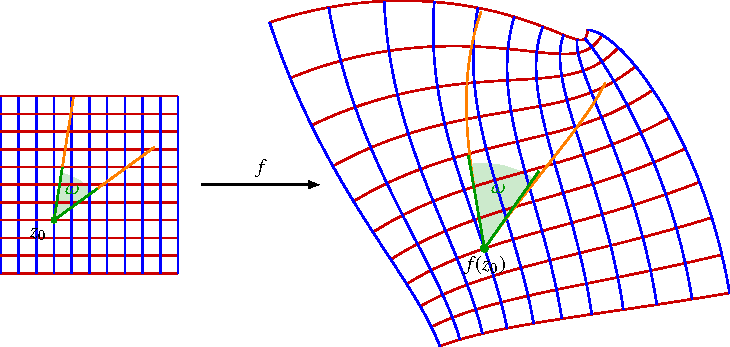
\includegraphics{chapters/020-holomorph/images/konform.pdf}
\caption{Eine holomorph Abbildung $f\colon \mathbb{C}\to\mathbb{C}$
ist konform.
Geraden mit Richtung $w\in\mathbb{C}$, $|w|=1$, durch den Punkt $z_0$
werden auf Kurven ({\color{orange}orange}) durch den Punkt $f(z_0)$
abgebildet, deren Tangenten ({\color{darkgreen}grün}) die Richtung
von $f'(z_0)\cdot w$ haben.
Die Multiplikation mit $f'(z_0)$ ist eine Drehstreckung, die Winkel
erhält.
\label{buch:holomorph:fig:konform}}
\end{figure}
%
Wir betrachten eine holomorphe Abbildung $f\colon U\to\mathbb{C}$ einer
offenen Menge nach $\mathbb{C}$.
Ein Punkt $z_0 \in U$ wird auf $f(z_0)\in\mathbb{C}$ abgebildet.
Die Abbildung~\ref{buch:holomorph:fig:konform} zeigt eine solche Abbildung.
Eine Gerade durch den Punkt $z_0$ kann durch die Richtung $d\in\mathbb{C}$
mit $|d|=1$ geschrieben werden.
Die Gerade besteht aus den Punkten $z_0+dt$ mit $t\in\mathbb{R}$.
Die Bildkurven sind $t\mapsto f(z_0+dt)$.
Die Tangente an die Bildkurve im Punkt $f(z_0)$ hat gemäss der
Ableitung  die Richtung von
\[
f'(z_0) \cdot d.
\]
Da Multiplikation mit $f'(z_0)$ eine Drehstreckung beschreibt, werden
Geraden durch $z_0$, die einen Winkel $\omega$ einschliessen, auf zwei
Tangenten abgebildet, die ebenfalls den Winkel $\omega$ einschliessen.
Folglich bleiben Winkel bei der Abbildung $f$ erhalten, sie ist
\emph{winkeltreu}.
\index{winkeltreu}%

\begin{definition}[konforme Abbildung]
Eine Abbildung, die in jedem Punkt winkeltreue ist,
heisst \emph{konform}.
\index{konform}%
\end{definition}

\begin{satz}
Eine holomorphe Funktion $f\colon U\to\mathbb{C}$ beschreibt in jedem
Punkt $z$, in dem $f'(z)\ne 0$ ist, eine konforme Abbildung.
\end{satz}

Die Gitterlinien stehen im Definitionsgebiet senkrecht aufeinander.
Die rechten Winkel werden von $f$ auf rechte Winkel zwischen den
Bildkurven der Gitterlinien abgebildet.
Daher schneiden sich die Gitterlinien in
Abbildung~\ref{buch:holomorph:fig:konform}
orthogonal.

%
% Nullstellen der Ableitung
%
\subsubsection{Nullstellen der Ableitung}
Bei einer Nullstelle von $f'(z_0)$ sind die Tangentenrichtungen der 
Bildkurven nicht definiert.
Entsprechend ist es nicht sinnvoll davon zu sprechen, dass Winkel bei
der Abbildung erhalten bleiben.
Die Abbildung $z\mapsto f(z) = z^n$ hat in Polarkoordinaten die
Darstellung 
\[
f(re^{i\varphi})
=
r^n e^{in\varphi}
=
r^n(\cos n\varphi + i\sin n\varphi).
\]
Geraden durch den Nullpunkt mit Polarwinkel $\varphi$ werden auf
Geraden durch den Nullpunkt mit Polarwinkel $n\varphi$ abgebildet.
Winkel im Nullpunkt werden also mit $n$ multipliziert.

Wir werden später zeigen, dass eine holomorphe Funktion auch eine 
konvergente Potenzreihe hat.
Hat die Ableitung $f'(z)$ eine Nullstelle im Punkt $z_0$, dann hat
$ g(z) = f(z) - f(z_0) $
eine Potenzreihe, die mit
\[
g(z)
=
\frac{f''(z_0)}{2!}(z-z_0)^2 + o((z-z_0)^2)
\]
beginnt.
Im Punkt $z_0$ werden Winkel daher mit $2$ multipliziert.
Ist die $n$-te Ableitung von $f$ die erste, die im Punkt $z_0$
nicht verschwindet, dann hat $g(z)$ die Potenzreihe
\[
g(z)
=
\frac{f^{(n)}(z_0)}{n!}(z-z_0)^n + o((z-z_0)^n).
\]
Winkel im Punkte $z_0$ werden also mit $n$ multipliziert.

Verwendet man als Definitionsgebiet
$U = \mathbb{C}\setminus\{x\in\mathbb{R} \mid x < 0\}$,
dann kann $z\mapsto f(z)=z^\alpha$ für beliebige rationale $\alpha>0$
durch die Polarformel $f(re^{i\varphi})=r^\alpha e^{i\alpha\varphi}$
definiert werden.
Winkel im Punkt $0$ werden mit $\alpha$ multipliziert.

%
% Winkeltreue Abbildungen sind holomorph
%
\subsubsection{Winkeltreue, orientierungserhaltende Abbildungen sind holomorph}
Eine differenzierbare Abbildung von $U\subset\mathbb{R}^2$ nach $\mathbb{R}^2$
hat die jacobische Matrix $\Jf$ als Ableitung.
Der Winkel zwischen den beiden Vektoren $\vec{u}$ und $\vec{v}$ und
zwischen den Bildvektoren ist
\begin{equation}
\cos
\angle(\vec{u},\vec{v})
=
\frac{\vec{u}\cdot\vec{v}}{|\vec{u}|\cdot |\vec{v}|}
\qquad\text{bzw.}\qquad
\cos
\angle(\Jf \vec{u},\Jf \vec{v})
=
\frac{\Jf \vec{u}\cdot \Jf \vec{v}}{|\Jf\vec{u}|\cdot |\Jf\vec{v}|}.
\label{buch:holomorph:geometrie:coswinkel}
\end{equation}
Sie ist genau dann winkeltreu, wenn die Matrix $\Jf$ das Skalarprodukt
nur mit einem skalaren Faktor $s$ multipliziert, denn dann bleibt der
Kosinus in \eqref{buch:holomorph:geometrie:coswinkel} und damit auch
der Winkel gleich.
Dies ist gleichbedeutend mit der Matrixgleichung
\[
\Jf^t I \Jf
=
\Jf^t \Jf
=
sI
\qquad\Rightarrow\qquad
\biggl(\frac{1}{\!\sqrt{s}}\Jf\biggr)^t
\biggl(\frac{1}{\!\sqrt{s}}\Jf\biggr)
=
I.
\]
Die Matrix
\[
A = \frac{1}{\!\sqrt{s}}\Jf
=
\frac{1}{\!\sqrt{s}}
{\renewcommand{\arraystretch}{2.0}
\begin{pmatrix}
\displaystyle\frac{\partial u}{\partial x} &
\displaystyle\frac{\partial u}{\partial y} \\
\displaystyle\frac{\partial v}{\partial x} &
\displaystyle\frac{\partial v}{\partial y}
\end{pmatrix}}
\]
muss also orthogonal sein.
Ein orthogonale Matrix in zwei Dimensionen ist aber eine Drehtmatrix
oder eine Drehmatrix mit nachfolgender Spiegelung, die die Orientierung
umkehrt.
Falls $\frac{1}{\!\sqrt{s}}\Jf$ eine Drehmatrix ist, folgt
\begin{align}
\frac{1}{\!\sqrt{s}}
{\renewcommand{\arraystretch}{2.0}
\begin{pmatrix}
\displaystyle\frac{\partial u}{\partial x} &
\displaystyle\frac{\partial u}{\partial y} \\
\displaystyle\frac{\partial v}{\partial x} &
\displaystyle\frac{\partial v}{\partial y}
\end{pmatrix}}
&=
\begin{pmatrix}
\cos\varphi&-\sin\varphi\\
\sin\varphi&\phantom{-}\cos\varphi
\end{pmatrix}
\quad\Rightarrow\quad
\left\{
\renewcommand{\arraycolsep}{1.5pt}
\begin{array}{rcccl}
\displaystyle
\frac{\partial u}{\partial x}
&=&
\!\sqrt{s}\cos\varphi
&=&
\displaystyle
\frac{\partial v}{\partial y}
\\[8pt]
\displaystyle
\frac{\partial v}{\partial x}
&=&
\!\sqrt{s}\sin\varphi
&=&
\displaystyle
-\frac{\partial u}{\partial y}
\end{array}
\right.
\label{buch:holomorph:gemetrie:eqn:JfCR}
\end{align}
Die Gleichungen auf der rechten Seite von
\eqref{buch:holomorph:gemetrie:eqn:JfCR}
sind die Cauchy-Riemann-Differential\-glei\-chun\-gen.
\index{Cauchy-Riemann-Differentialgleichungen}%
Damit haben wir den folgenden Satz bewiesen.

\begin{satz}
Ist 
\[
F
\colon
U \to \mathbb{R}^2
:
(x,y) \mapsto \begin{pmatrix} u(x,y)\\v(x,y)\end{pmatrix}
\]
eine differenzierbare Abbildung, die orientierungserhaltend und
winkeltreu ist.
Dann ist die Funktion $f(x+iy) = u(x,y) + iv(x,y)$ eine holomorphe
Funktion.
\end{satz}


%
% 22-riemann.tex -- Der Abbildungssatz von Riemann
%
% (c) 2026 Prof Dr Andreas Müller
%
\subsection{Der Abbildungssatz von Riemann}
Isometrische Abbildungen sind konform, bilden aber ein Gebiet immer
auf ein kongruentes Gebiet ab.
Ähnlichkeitsabbildungen bilden ein Gebiet immer auf ein ähnliches
Gebiet ab.
In beiden Fällen gibt es einen sehr einfachen Zusammenhang zwischen
Urbildmenge und Bildmenge, es ist leicht zu entscheiden,
ob eine Abbildung zuwischen zwei Mengen existiert.

Die Menge der konformen Abbildung ist jedoch viel grösser,
mithilfe holomorpher Abbildungen lassen sich Abbildungen
zwischen sehr viel allgemeineren Gebieten der komplexen Ebene
konstruieren.
Wir definieren den folgenden Begriff, um die Idee der
bijektiven, winkeltreuen und orientierungserhaltenden Abbildung
für komplexe Funktionen zu kodifizieren.

\begin{definition}[biholomorph]
Sind $U$ und $V$ offene Mengen in $\mathbb{C}$, dann heisst
eine Abbildung $f\colon U\to V$ \emph{biholomorph}, wenn sie bijektiv
und holomorph ist.
\index{biholomorph}%
\end{definition}

%
% Die obere Halbebene und Polygone
%
\subsubsection{Die obere Halbebene und Polygone}
Die Abbildung $z\mapsto z^\alpha$ ist holomorph auf der oberen Halbebene
\[
H = \{z\in\mathbb{C}\mid \operatorname{Im}z> 0\}.
\]
\index{obere Halbebene}%
\index{Halebene, obere}%
Sie bildet die reelle Achse auf zwei Geraden ab, die den Winkel $\alpha \pi$
einschliessen.
Durch Zusammensetzen solcher Abbildungen lässt sich eine Abbildung
der oberen Halbebene auf ein Polygon konstruieren.

\begin{definition}[Schwarz-Christoffel-Transformation]
Für reelle Zahlen $a_k$ mit $a_1<a_2<\dots<a_n$, Winkel
$\alpha_1,\dots,\alpha_n\in\mathbb{R}$ und eine Konstante $K\in \mathbb{C}$
heisst die auf der oberen Halbebene definierte Abbildung
\[
z
\mapsto 
f(z)
=
\int^z \frac{K}{
(w-a_1)^{1-\alpha_1/\pi}
(w-a_2)^{1-\alpha_2/\pi}
\dots
(w-a_n)^{1-\alpha_n/\pi}
}\,dw
\]
die Schwarz-Christoffel-Transformation.
\index{Schwarz-Christoffel-Transformation}%
\end{definition}

Die Schwarz-Christoffel-Transformation ist nur bis auf eine
Integrationskonstante definiert.
Ebenso muss man bei der Berechnung der Potenzen $(w-a_k)^{1-\alpha k/\pi}$
im Nenner eine geeignete Fortsetzung der Potenzfunktion wählen, damit
eine holomorphe Funktion entsteht.

Man kann zeigen, dass die Schwarz-Christoffel-Transformation die reelle Achse
auf ein Polygon mit Innenwinkeln $\alpha_1$ an der Stelle $f(a_i)$ abbildet.
Die Konstante $K$ kann dazu verwendet werden, das Polygon beliebig zu drehen
und zu skalieren.
Durch Wahl einer geeigneten Integrationskonstante kann das Polygon an
jede beliebige Stelle der komplexen Ebene verschoben werden.

Ein bekannter Spezialfall der Schwarz-Christoffel-Transformation ist
das elliptische Integral
\begin{align*}
f(z)
&=
\int^z
\frac{1}{\!\sqrt{(1-w^2)(1-k^2w^2)}}\,dw
\\
&=
\int^z 
\frac{1/k^2}{\!\sqrt{(w^2-1)(k^2w^2-\frac{1}{k^2})}}\,dw
\\
&=
\int^z
\frac{1/k^2}{
(w-1)^{1-\frac12}
(w-\frac{1}{k})^{1-\frac12}
(w+\frac{1}{k})^{1-\frac12}
(w+1)^{1-\frac12}
}\,dw.
\end{align*}
mit $0<k<1$.
Die Bildmenge ist ein Polygon mit 5 Ecken und Winkeln $90^\circ$-Winkeln
in den Ecken $f(\pm 1)$ und $f(\pm\frac{1}{k})$.
Da die Winkelsumme in einem 5-Eck $540^\circ$ ist, muss der Winkel
an der Ecke $\lim_{z\to\infty}f(z)$ $180^\circ$ sein.
Mehr Information zur Theorie der elliptischen Integrale findet der
interessierte Leser in Kapitel~\ref{chapter:elliptisch}.

Das Beispiel der elliptischen Integrale zeigt, dass man nicht erwarten
kann, die Transformation in geschlossener Form auszuführen.
Für die numerische Rechnung ist die Definition durch die Differentialgleichung
\[
\frac{f''(z)}{f'(z)}
=
\sum_{k=1}^n \frac{\alpha_k-1}{z-a_k}
\]
oft zugänglicher.
In Matlab steht ein Paket zur Verfügung, welches die
Schwarz-Christoffel-Transformation durch interaktive Wahl der Eckpunkte
des Polygons zu konstruieren gestattet.
\index{Matlab}%
Sie wird in Kapitel~\ref{chapter:elektro} verwendet.

%
% Der riemannsche Abbildungssatz
%
\subsubsection{Der riemannsche Abbildungssatz}
Die Schwarz-Christoffel-Transformation ist eine diskrete Approxomation
des folgenden allgemeine Satzes, der zum ersten Mal von
Bernhard Riemann
\index{Riemann, Bernhard}%
in seiner Dissertation formuliert wurde.

\begin{definition}[Einheitskreisscheibe]
Die \emph{Einheitskreisscheibe} in der komplexen Ebene ist die offene Menge
\[
D
=
\{
z\in\mathbb{C}
\mid
|z|<1
\}.
\]
\end{definition}

\begin{satz}[Riemann]
\label{buch:holomorph:riemann:satz:riemann}
Ist $U$ ein einfach zusammenhängendes Gebiet in $\mathbb{C}$, welches nicht
ganz $\mathbb{C}$ ist, dann gibt es eine biholomorphe Abbildung
$f\colon U\to D$ von $U$ auf die Einheitskreisscheibe.
Die Abbildung ist eindeutig bestimmt, wenn zusätzlich von einem Punkt
$z_0\in H$ gefordert wird, dass $f(z_0)=0$ und $f'(z_0)>0$ verlangt wird.
\end{satz}

Der von Riemann in seiner Dissertation im Jahr 1851 gegeben Beweis
wurde später von Weierstrass als unvollständig erkannt.
\index{Weierstrass, Karl}%
Den ersten vollständigen Beweis gab William Fogg Osgood erst 1900.
\index{Osgood, William Fogg}%
Ein Beweis würde den Rahmen dieses Seminars sprengen, viele Standardwerke
über komplexe Analysis wie \cite{buch:alfohrs,buch:lang} enthalten
Beweise des Satzes.

Auch die Einheitskreisscheibe erfüllt die Voraussetzungen des Satzes.
Drehungen $z \mapsto f(z)=e^{i\varphi} z$ bilden $D$ biholomorph auf $D$ ab.
Die Forderung $f'(z)=e^{i\varphi}>0$ in der Formulierung des
Satzes~\ref{buch:holomorph:riemann:satz:riemann}
bedeutet, dass $\varphi=0$ sein muss,
sie schliesst also Drehungen aus.

Für $z_0\in D$ ist die Abbildung
\begin{equation}
z
\mapsto
f(z)
=
e^{i\varphi}\frac{z-z_0}{1-\bar{z}_0z}
\label{buch:holomorph:geometrie:automorphD}
\end{equation}
als rationale Funktion holomorph.
Sie bildet $z_0$ auf den Nullpunkt ab.
Für einen Punkt $z$ auf dem Rand von $D$ ist $|z|=1$ und daher.
\[
1-\bar{z}_0z
=
|z|^2-\bar{z}_0z
=
\bar{z}z-\bar{z}_0z
=
(\bar{z}-\bar{z}_0)z.
\]
Dies bedeutet, dass $f(z)$ den Betrag
\[
|f(z)|^2
=
\frac{|z-z_0|^2}{|1-\bar{z}_0z|^2}
=
\frac{|z-z_0|^2}{|(\bar{z}-\bar{z}_0)z|^2}
=
\frac{|z-z_0|^2}{|\bar{z}-\bar{z}_0|^2\,|z|^2}
=
\frac{|z-z_0|^2}{ |z-z_0|^2}
=
1
\]
hat.
Der Rand von $D$ wird also wieder auf den Rand von $D$ abgebildet.
Der Faktor $e^{i\varphi}$ fügt eine Drehung um den Winkel $\varphi$ hinzu.
Sie ist auch umkehrbar:
\begin{align*}
w &= e^{i\varphi}\frac{z-z_0}{1-\bar{z}_0z}
&&\Rightarrow&
we^{-i\varphi}(1-\bar{z}_0z) &= z-z_0
\\
&&&&
we^{-i\varphi} + z_0 &= z+we^{-i\varphi}\bar{z}_0z
\\
&&&&
we^{-i\varphi} + z_0 &= z(1+we^{-i\varphi}\bar{z}_0)
\\
&&&&
z&=
\frac{1+we^{-i\varphi}\bar{z}_0}{ we^{-i\varphi} + z_0}.
\end{align*}
Poincaré hat gezeigt, dass jede biholomorphe Selbstabbildung von $D$
die Form \eqref{buch:holomorph:geometrie:automorphD} hat.
Dies erklärt, warum die Zusatzbedingung des Satzes von Riemann, dass
$z_0\in U$ auf $0$ abgebildet werden muss, die Abbildung eindeutig macht.

Die obere Halbebene $H$ erfüllt die Voraussetzungen des riemannschen
Abbildungssatzes.
Er garantiert, dass es eine Abbildung $f\colon H\to D$ der oberen
Halbebene auf die Einheitskreisscheibe gibt.
Eine solche kan als Möbius-Transformation gefunden werden, wie in
Kapitel~\ref{chapter:moebius} gezeigt wird.
Auch ein Polygon $P$ in der komplexen Ebene erfüllt die Bedingungen,
somit gibt es auch ein biholomorphe Abbildung des Polygons auf die
Einheitskreisscheibe.
Die Zusammensetzung $g^{-1}\circ f$ ist dann eine biholomorphe Abbildung
der oberen Halbebene auf das Polygon.
Die Schwarz-Christoffel-Transformation ist eine explizite Formel
für diese Abbildung.

%
% 23-anwendungen.tex -- Anwendungen
%
% (c) 2026 Prof Dr Andreas Müller
%
\subsection{Anwendungen
\label{buch:holomorph:geometrie:subsection:anwendungen}}
Konforme Abbildungen ermöglichen, komplizierte Gebiete auf 
komplex differenzierbare Art auf sehr einfache Gebiete abzubilden.
Zum Beispiel kann man nach einer harmonischen Funktion mit 
gegebenen Randwerten auf dem Gebiet fragen.
Die konforme Abbildung macht daraus das Problem, eine harmonische
Funktion auf einem Kreisgebiet mit gegebenen Randwerten zu finden.
Für Lösung dieses Problem gibt es aber sogar eine Formel von Poisson.
Durch Zusammensetzen der Lösung von Poisson mit der konformen
Abbildung entsteht eine Lösung des schwierigen Problems auf dem
ursprünglichen Gebiet.

Diese Idee, durch Abbildung des Gebietes eine Aufgabenstellung
auf eine bereits gelöste Aufgabe zu transformieren, wird in
zwei weiteren Kapiteln dieses Seminars verwendet.
In Kapitel~\ref{chapter:elektro} wird die Elektrostatik in der
Ebene untersucht.
Da in der Elektrostatik alles durch das elektrostatische Potential
gegeben ist, genügt es Potentialfunktionen zu finden.
Für komplexe Geometrie der berandenden Leiter kann dies eine
sehr schwierige Aufgabe sein.
Das Potential eines unregelmässigen Körpers kann aber durch
eine Abbildung der Ebene ausserhalb des Körpers auf das
äussere der Einheitskreisscheibe gefunden werden,
da das Potential eines Kreises $\sim\frac1r$ ist.

Zweidimensionale laminare Strömungen lassen sich durch die sogenannte
Stromfunktion beschreiben, die eine harmonische Funktion ist.
Es ist jedoch im allgemeinen schwierig, diese Funktion für eine
komplexe Geometrie des umströmten Körpers, zum Beispiel eines Flügelprofils,
zu finden.
Für die Umströmung eines Kreises kann man jedoch eine Formel
angeben.
Es muss jetzt nur noch eine Abbildung des Aussenraumes des Flügelprofils
auf den Aussenraum des Kreises gefunden werden.
Diese Idee ermöglicht sogar eine Formel für den Auftrieb eines Flügels
herzuleiten, sie wird in Kapitel~\ref{chapter:joukowski} genauer
ausgeführt.



